\documentclass[11pt,twocolumn]{article}

\usepackage{cmap} % Generates ToUnicode mapping tables for PDF text extraction
% --- Core packages ---
\usepackage[utf8]{inputenc}
\usepackage[T1]{fontenc}
\usepackage{lmodern}  % Latin Modern fonts: provides proper ToUnicode CMaps for PDF text extraction
\usepackage{amsmath,amssymb,amsfonts,amsthm}
\usepackage{mathtools}
\usepackage{bm}
\usepackage{graphicx}
\usepackage{booktabs}
\usepackage{tabularx}
\usepackage{multirow}
\usepackage{enumitem}
\usepackage{hyperref}
\usepackage{cleveref}
\usepackage{xcolor}
\usepackage{microtype}
\usepackage{algorithm}
\usepackage{algpseudocode}
\usepackage[margin=0.85in]{geometry}
\usepackage{caption}
\usepackage{subcaption}
\usepackage{float}
\usepackage{listings}
\usepackage{stfloats} % Stabilizes two-column floats and prevents text overlap anomalies

% --- Code listing style (ensures reliable glyph rendering for copy-paste) ---
\lstset{
  language=Python,
  basicstyle=\footnotesize\ttfamily,
  columns=flexible,
  keepspaces=true,
  breaklines=true,
  frame=none,
  xleftmargin=1em,
  showstringspaces=false,
  commentstyle=\itshape\color{gray},
}

\hypersetup{
  colorlinks=true,
  linkcolor=blue!70!black,
  citecolor=green!50!black,
  urlcolor=blue!60!black
}

\newcommand{\simplex}{\mathcal{S}}
\newcommand{\closure}{\mathcal{C}}
\newcommand{\R}{\mathbb{R}}
\newcommand{\N}{\mathcal{N}}

\title{Automated Code-Guided Chart Synthesis and Visual Degradation:\\
A Unified Framework for Multimodal Document Parsing\\
and Visual Reasoning Benchmarks}

\author{
  Gabriel S Stuart\thanks{Correspondence: gabrielst13@outlook.com}
}

\date{}

\begin{document}
\maketitle

% ============================================================
%  ABSTRACT
% ============================================================
\begin{abstract}
Multimodal large language models (MLLMs) and visual document parsers demand large, structurally diverse datasets that capture the interplay of text, categorical hierarchies, and graphical primitives.
Crowdsourced annotation scales poorly and introduces systematic spatial-coordinate errors.
We present a code-guided chart synthesis framework that couples explicit mathematical data-generation engines to graphical layout compilers across scientific and business domains, producing bar, line, box plot, heatmap, pie, histogram, scatter, and area charts with pixel-perfect ground-truth coordinates, scene graphs, and multi-keypoint pose schemas.
To close the domain gap between clean digital renderings and real-world scanned documents, vector outputs pass through a post-rendering degradation pipeline applying perspective homography, multi-channel chromatic aberration, directional blur, and non-uniform lighting.
The framework incorporates Tufte's~\cite{tufte2001} graphical-integrity principles, minimizing non-data ink and analyzing coordinate-space prerequisites for non-linear scale verification.
\end{abstract}

\smallskip
\noindent\textbf{Keywords:} Code-Guided Synthesis, Multimodal Large Language Models, Visual Encodings, Computational Visualization, Image Degradation Frameworks, Spatial Ground Truth.

% ============================================================
%  1. INTRODUCTION
% ============================================================
\section{Introduction}\label{sec:intro}

Data-visualization interpretation is a demanding benchmark for visual reasoning: it requires joint textual OCR, structural orientation tracking, coordinate-scale matching, and multi-step quantitative inference.
Crowdsourced annotation datasets scale poorly and suffer from bounding-box inaccuracies that degrade training of networks aimed at precise numerical extraction from dense charts.
Code-guided synthesis pipelines sidestep these limitations by programmatically linking data frames to visual styles, creating a direct channel from data tables to graphic components.
This strategy underpins recent vision-language benchmarks: ChartNet~\cite{kondic2026chartnet} and ChartMaster~\cite{liu2026chartmaster} compile databases into executable rendering configurations; ChartGemma~\cite{masry2024chartgemma} pairs web-harvested tables with programmatic charts for instruction tuning; and ChartGen~\cite{kondic2025chartgen} scales chart understanding through synthetic generators.
ChartQAPro~\cite{masry2025chartqapro} and EncQA~\cite{han2026encqa} probe visual encodings and complex multi-step reasoning over dense layouts.
Synthesize Step-by-Step~\cite{li2024synthesize} uses template-driven code abstractions for question--answer pair generation, DreamStruct~\cite{peng2024dreamstruct} bootstraps visual datasets from structural specifications, and Chart2Text-Enriched~\cite{suh2025chart2text} benchmarks fine-grained, context-aware chart summarization.

Training exclusively on clean digital vectors leaves a substantial domain gap.
Real-world documents undergo print-and-scan degradation, hand-held camera perspective warping, lens defocus, and sensor noise.
Synthetic pipelines must therefore apply post-rendering degradation that simulates physical defects while propagating updates to all internal spatial-coordinate annotations.
Table~\ref{tab:pipeline_comparison} summarizes existing chart synthesis pipelines.

\begin{table}[htbp]
\centering
\caption{Comparison of synthetic chart generation pipelines.}\label{tab:pipeline_comparison}
\scriptsize
\setlength{\tabcolsep}{3pt}
\begin{tabular}{@{} l c c c c @{}}
\toprule
\textbf{Pipeline} & \textbf{Deg.} & \textbf{Coord.} & \textbf{Kpts} & \textbf{Prof.} \\
\midrule
ChartNet~\cite{kondic2026chartnet}     & --      & --         & --         & Gen. \\
ChartGemma~\cite{masry2024chartgemma}  & --      & --         & --         & Web \\
ChartGen~\cite{kondic2025chartgen}     & Limited & --         & --         & Gen. \\
\textbf{Ours}                          & \textbf{Full} & \textbf{W/R} & \textbf{5/51} & \textbf{S/B} \\
\bottomrule
\end{tabular}
\end{table}

This paper describes a code-guided visualization synthesis and image degradation architecture.
We show how Tufte's~\cite{tufte2001} non-data-ink minimization principles---realized through themes such as \texttt{minimal} and \texttt{prism}---translate into Matplotlib~\cite{hunter2007matplotlib} and Seaborn~\cite{waskom2021seaborn} rendering configurations.
We formalize the system's design parameters, derive the coordinate-space transformations required for non-linear scale verification, and document the geometric warp profiles used to build robust visual document reasoning benchmarks.

% ============================================================
%  2. PIPELINE ARCHITECTURE & DOMAIN TAXONOMY
% ============================================================
\section{Pipeline Architecture \& Domain Taxonomy}\label{sec:architecture}

The framework organizes chart rendering through a unified configuration hierarchy, partitioning parameters across two application profiles so that categorical taxonomies, noise bounds, and presentation themes reflect the distinct conventions of technical journals and corporate dashboards.

\subsection{The Scientific Profile}\label{sec:scientific}

The scientific profile emulates experimental measurements, biological assays, and clinical outcomes.
The text engine draws from over 100 professional measurement combinations (\texttt{SCIENTIFIC\_DOMAIN\_DICT}), injecting axis labels such as \emph{Reads per million (RPM)}, \emph{Dissociation Constant ($K_{\text{d}}$, nM)}, \emph{Optical Density ($OD_{600}$)}, \emph{Molarity (mM)}, \emph{Fold Change}, and \emph{NMR Chemical Shift (ppm)}.
Categorical markers draw from authentic biological vocabularies: common oncogenes (TP53, BRCA1, BRCA2, EGFR, KRAS) and signaling pathways (PI3K-AKT, MAPK, WNT, Apoptosis).
The profile enforces high-precision error bars, statistical significance brackets, and skewed or zero-inflated density structures that reflect realistic instrumentation baselines.

\subsection{The Business Profile}\label{sec:business}

The business profile targets corporate analytics, KPIs, and economic reporting.
Text strings map to enterprise metric taxonomies (\texttt{BUSINESS\_DOMAIN\_DICT}): \emph{Monthly Active Users (MAU)}, \emph{Customer Lifetime Value (LTV~\$)}, \emph{Cost per Acquisition (CAC~\$)}, \emph{Net Promoter Score (NPS)}, and \emph{EBITDA~(\$)}.
Categorical labels draw from organizational records: product SKUs, billing cycles, fulfillment timelines, and geographic sales regions.
Structurally, this profile emphasizes multi-component seasonal trends, exponential adoption curves with market ceilings, and clean monochromatic or corporate-accented palettes.

% ============================================================
%  3. MATHEMATICAL DATA GENERATION ENGINES
% ============================================================
\section{Mathematical Data Generation Engines}\label{sec:math}

Rather than drawing from flat uniform distributions, the framework samples continuous tracks from explicit mathematical equations parameterized to model realistic natural phenomena and business processes.

\subsection{Dose--Response Curves (The Hill Equation)}\label{sec:hill}

Drug efficacy and cellular dose--response transitions are modeled as a sigmoidal function derived from the Hill equation~\cite{hill1910dissociation}:
\begin{equation}\label{eq:hill}
  \text{data} = \text{baseline} + \frac{\text{max\_response} \mathbin{\text{-}} \text{baseline}}{1 + 10^{h(\text{ec50} \mathbin{\text{-}} \log_{\text{conc}})}},
\end{equation}
where concentration spans pM to mM scales ($\log_{\text{conc}} \in [\text{-}10, \text{-}3]$), the inflection midpoint $\text{ec}_{50} \sim \mathcal{U}(\text{-}8.5, \text{-}4.5)$, and the cooperativity coefficient $h$ varies as $\mathcal{U}(0.7, 1.3)$ for single-site binding, $\mathcal{U}(1.3, 2.0)$ for cooperative transitions, and $\mathcal{U}(2.0, 3.5)$ for high-cooperativity regimes.

Measurement noise is non-uniform, scaling with the local slope via heteroscedastic error modeling after Rodbard~\cite{rodbard1974statistical}. The coefficient of variation peaks near inflection thresholds where the response fraction $r_f$ changes most rapidly, replicating immunoassay and bioassay variance profiles:
\begin{align}
  \text{cv} &= 0.05 + 0.10\sqrt{r_f \cdot (1 \mathbin{\text{-}} r_f)}, \label{eq:cv}\\
  \text{noise} &\sim \N\!\bigl(0,\;(\text{data} \cdot \text{cv})^2\bigr), \label{eq:hill_noise}
\end{align}
where $r_f = (\text{data} - \text{baseline})\,/\,(\text{max\_resp} - \text{baseline})$.

\subsection{Biological \& Technical Replicates}\label{sec:replicates}

Variability across independent cell populations is modeled with an asymmetric log-normal distribution rather than symmetric Gaussian noise, since biological replication error accumulates multiplicatively~\cite{limpert2001lognormal}:
\begin{align}
  \sigma &= \sqrt{\log_e\bigl(1 + \text{CV}_{\text{target}}^2\bigr)}, \label{eq:lognorm_sigma}\\
  \mu &= \log_e(\text{mean\_val}) \mathbin{\text{-}} 0.5\,\sigma^2, \label{eq:lognorm_mu}\\
  \text{data} &\sim \exp\bigl(\N(\mu, \sigma^2)\bigr). \label{eq:lognorm}
\end{align}

The target $\text{CV}_{\text{target}}$ matches validated laboratory protocol baselines from the Eli Lilly and NCATS immunoassay guidelines~\cite{lilly2012immunoassay}, constraining generative noise envelopes to realistic clinical ranges. Protocol-specific targets are listed in Table~\ref{tab:cv_baselines}.

\begin{table*}[t]
\centering
\caption{Empirical CV Baseline Envelopes (verified against Eli Lilly~\cite{lilly2012immunoassay}).}\label{tab:cv_baselines}
\small
\begin{tabularx}{\textwidth}{l c X}
\toprule
\textbf{Assay Platform / Protocol} & \textbf{Empirical CV} & \textbf{Primary Physical Mechanism of Variation} \\
\midrule
Quantitative PCR (qPCR) & $5\% - 15\%$ & Amplification efficiency drift, micro-volume pipetting errors \\
Western Blot & $10\% - 25\%$ & Membrane binding variance, transfer efficiency fluctuations \\
Dynamic Cell Microplates & $15\% - 35\%$ & Ambient edge effects, localized evaporation, temperature gradients \\
\bottomrule
\end{tabularx}
\end{table*}

\subsection{Exponential Decay and Pharmacokinetic Clearance}\label{sec:decay}

Chemical clearance or radioactive isotope degradation is simulated across a temporal vector $t$:
\begin{align}
  \text{data} &= (\text{init} \mathbin{\text{-}} \text{baseline}) \cdot e^{\text{-}k \cdot t} + \text{baseline}, \label{eq:decay}\\
  k &= \frac{\log_e 2}{t_{1/2}}, \qquad t_{1/2} \in [0.5,\, 72]~\text{hours}. \label{eq:halflife}
\end{align}
A proportional error envelope overlays the sequence:
\begin{equation}\label{eq:decay_noise}
  \text{noise} \sim \N\bigl(0,\; (\text{data} \cdot 0.08 + 0.02 \cdot \text{max\_scale})^2\bigr).
\end{equation}

\subsection{Enzyme Kinetics (Michaelis--Menten)}\label{sec:mm}

Initial reaction velocities under varying substrate concentrations follow the Michaelis--Menten hyperbolic model~\cite{michaelis1913kinetik}:
\begin{equation}\label{eq:mm}
  \text{data} = \frac{V_{\max} \cdot [\text{S}]}{K_m + [\text{S}]},
\end{equation}
where $V_{\max}$ is the maximum velocity and $K_m$ the Michaelis constant. Measurement noise follows $\text{CV} \in [0.05, 0.15]$, consistent with analytical chemistry quality-control standards.

\subsection{Spectroscopy \& Chromatography Peaks}\label{sec:peaks}

Mass spectrometry and chromatography elution profiles are modeled as Gaussian peaks:
\begin{equation}\label{eq:gauss_peak}
  \text{data} = A \cdot \exp\!\biggl(-\frac{(x-\mu)^2}{2\sigma^2}\biggr) + \text{baseline}.
\end{equation}
This follows Martin and Synge's~\cite{martin1941new} partition theory, in which multi-stage partitioning produces approximately Gaussian elution profiles. Poisson-like photon-counting noise replicates detector physics:
\begin{equation}\label{eq:poisson_noise}
  \text{noise} \sim \N\!\Bigl(0,\;\bigl(0.3\sqrt{|\text{data}-\text{baseline}|}\bigr)^2\Bigr).
\end{equation}

\subsection{Compositional Data Models (The Aitchison Simplex)}\label{sec:simplex}

Proportional charts represent data constrained to the Aitchison simplex~\cite{aitchison1986statistical}:
\begin{equation}\label{eq:simplex}
  \simplex^D = \Bigl\{\mathbf{x} \in \R^D \;\Big|\; x_i > 0,\; x_1 + \dots + x_D = 1\Bigr\}.
\end{equation}
Aitchison showed that proportional data require log-ratio transformations to avoid spurious correlations and scale-dependent artifacts.

\paragraph{Closure ($\closure$).} Projects any raw positive vector into the simplex:
\begin{equation}\label{eq:closure}
  \closure(\mathbf{x}) = \biggl[\frac{x_1}{\sum_k x_k},\;\frac{x_2}{\sum_k x_k},\;\ldots,\;\frac{x_D}{\sum_k x_k}\biggr].
\end{equation}

\paragraph{Perturbation ($\oplus$).} Compositional addition via component-wise multiplication followed by closure:
\begin{equation}\label{eq:perturbation}
  \mathbf{x} \oplus \mathbf{y} = \closure\bigl([x_1 y_1,\; x_2 y_2,\;\ldots,\; x_D y_D]\bigr).
\end{equation}

\paragraph{Power Transform ($\odot$).} Scalar multiplication on the simplex:
\begin{equation}\label{eq:power}
  \alpha \odot \mathbf{x} = \closure\bigl([x_1^\alpha,\; x_2^\alpha,\;\ldots,\; x_D^\alpha]\bigr).
\end{equation}

\paragraph{Aitchison Distance ($d_A$).} The log-ratio geometric distance, where $g(\mathbf{x}) = (\prod_i x_i)^{1/D}$:
\begin{equation}\label{eq:aitchison_dist}
  d_A(\mathbf{x}, \mathbf{y}) = \sqrt{\sum_{i=1}^D \left(\log_e\frac{x_i}{g(\mathbf{x})} - \log_e\frac{y_i}{g(\mathbf{y})}\right)^{\!2}}.
\end{equation}

\paragraph{Sampling Configurations.}
Slices ($D \in [3, 12]$) are generated via several methods:

\noindent\emph{Asymmetric Dirichlet:}
\begin{equation}\label{eq:dirichlet}
  f(\mathbf{x};\bm{\alpha}) = \frac{1}{\mathrm{B}(\bm{\alpha})}\prod_{i=1}^D x_i^{\alpha_i - 1},
\end{equation}
modified by an asymmetry trend factor ($\text{trend} \in [1.0-s,\;1.0+s]$, $s \in [0.0,\,1.5]$).

\noindent\emph{Stick-Breaking Process:} Following Sethuraman's constructive definition~\cite{sethuraman1994constructive}:
\begin{align}\label{eq:stickbreak}
  V_k &\sim \text{Beta}(1, \gamma),\;\gamma \in [1.0,8.0]; \nonumber\\
  x_k &= V_k\!\prod_{j=1}^{k-1}(1 - V_j).
\end{align}

\noindent\emph{Kummer--Dirichlet (Type~I Confluent) Sampling:}
Compositions are generated by drawing latent components $\mathbf{z}$ from independent standard Gamma distributions on the positive orthant $\R_+^D$:
\begin{equation}\label{eq:kdga_raw}
  g(\mathbf{z}) \propto \biggl(\prod_{i=1}^D z_i^{\alpha_i - 1}\biggr)\exp\biggl(-\sum_{i=1}^D z_i\biggr),\quad \mathbf{z} \in \R_+^D.
\end{equation}
Following Makgai, Bekker, and Arashi~\cite{makgai2021compositional}, each component is tilted via the non-linear transformation $w_i = z_i e^{-\lambda z_i}$ before closure onto $\simplex^D$:
\begin{equation}\label{eq:kdga_closure}
  \mathbf{x} = \closure\!\bigl([z_1 e^{-\lambda z_1},\;\dots,\;z_D e^{-\lambda z_D}]\bigr).
\end{equation}
Because this transformation is non-linear, it resists cancellation under closure, producing skewed compositional profiles with outliers. The parameter $\lambda \in [-3, 3]$ controls asymmetric deformation intensity; $\lambda = 0$ recovers the standard Dirichlet on $\simplex^D$.

\paragraph{Entropy-Loss Tail Aggregation.}
When slices exceed a threshold ($\text{max\_slices}=5$), low-weight components are collapsed into an ``Other'' category governed by Shannon entropy:
\begin{align}
  H(\mathbf{x}) &= -\sum_{i=1}^D x_i \log_2 x_i, \label{eq:entropy}\\
  \Delta H &= H(\mathbf{x}_{\text{orig}}) - H(\mathbf{x}_{\text{agg}}). \label{eq:entropy_loss}
\end{align}
If $\Delta H > 0.5$, consolidation terminates to preserve fine-grained structural data.

\subsection{Zero-Inflated Profiles for Histograms}\label{sec:zeroinflated}

Histogram observation pools ($N \in [300, 1200]$) are sampled across continuous and zero-inflated frameworks, drawing on single-cell genomics methodologies like MAST~\cite{finak2015mast}:

\noindent\emph{Gaussian Mixture Model (GMM):}
\begin{equation}\label{eq:gmm}
  f(x) = \sum_{k=1}^K w_k \cdot \frac{1}{\sigma_k\sqrt{2\pi}}\exp\biggl(-\frac{(x-\mu_k)^2}{2\sigma_k^2}\biggr),
\end{equation}
where $K \in [2,4]$ and weights $\mathbf{w}$ follow a uniform Dirichlet.

\noindent\emph{Weibull Distribution:}
\begin{equation}\label{eq:weibull}
  f(x) = \frac{c}{\lambda}\Bigl(\frac{x}{\lambda}\Bigr)^{c-1}\exp\biggl(-\Bigl(\frac{x}{\lambda}\Bigr)^c\biggr),\; c \in [0.8, 2.5].
\end{equation}

\noindent\emph{Zero-Inflated Gaussian (ZIG):} Bounded by zero-inflation thresholds:
\begin{equation}\label{eq:zig}
  X_i = \begin{cases}
    0 & \text{w.p. } \pi,\\
    \N(\mu,\sigma^2) & \text{w.p. } 1-\pi,
  \end{cases}\quad \pi \in [0.2, 0.6].
\end{equation}
The ZIG model (hurdle-normal) captures excess zeros from biological dropouts and detection limits, as characterized in single-cell frameworks such as MAST~\cite{finak2015mast}.

\subsection{Scatter Trend and Clustered Models}\label{sec:scatter}

Scatter tracks are mapped against target $R^2$ bounds, following correlation and covariance models based on Pearson~\cite{pearson1897mathematical}:

\noindent\emph{Linear Core:}
\begin{align}
  \mathbf{y}_{\text{perf}} &= m(\mathbf{x}-\bar{x}) + c, \label{eq:scatter_linear}\\
  \sigma_{\text{noise}}^2 &= \sigma_{\mathbf{y}_{\text{perf}}}^2 \cdot \frac{1-R^2}{R^2}, \label{eq:scatter_noise}\\
  y_i &= y_{\text{perf},i} + \N(0,\;\sigma_{\text{noise}}^2). \label{eq:scatter_final}
\end{align}
Noise variance is calibrated to achieve target $R^2$ values, preventing arbitrary scatter patterns.

\noindent\emph{Nonlinear Tracks:} Quadratic ($y = ax^2 + bx + c$), exponential ($y = a\exp(bx/\text{scale}) + c$), or logarithmic ($y = a\log_e(x+1)+c$) matrices with proportional CV noise ($\text{CV}_{\text{noise}} \in [0.08, 0.15]$).

\noindent\emph{Bivariate Multicluster Profiles:}
$K \in [2,3,4]$ clusters are generated via multivariate normals:
\begin{align}
  N_k &= \max\bigl(5,\;\lfloor N/K \rfloor + \mathcal{U}\{-3,3\}\bigr), \label{eq:cluster_size}\\
  \bm{\Sigma}_k &= \begin{bmatrix} \sigma_{xx} & \sigma_{xy}\\ \sigma_{xy} & \sigma_{yy}\end{bmatrix},\quad \rho \in [-0.5,\,0.5], \label{eq:cluster_cov}\\
  \mathbf{P}_{i,k} &\sim \N_2(\bm{\mu}_k,\;\bm{\Sigma}_k). \label{eq:cluster_sample}
\end{align}

\paragraph{Business-Domain Data Models.}
The business profile simulates transaction ledgers and corporate performance metrics using financial synthetic data techniques reviewed by Meldrum et al.~\cite{meldrum2025newmoney}, including multi-component seasonal waveforms and power-law Pareto distributions.

\subsection{Multi-Component Seasonality \& Trend}\label{sec:seasonal}

Macroeconomic timelines and consumer trends are simulated across fiscal calendars:
\begin{equation}\label{eq:seasonal}
  \text{data} = b + s \cdot x + \sum_{m}\bigl[a_m \cos(f_m x + \phi_m)\bigr],
\end{equation}
where the sub-component matrix $m$ concurrently evaluates annual periods ($f = 2\pi/12$) and quarterly cycles ($f = 2\pi/3$), and noise variance expands proportionally during peak seasonal waves.

\subsection{Saturated Exponential Growth}\label{sec:satgrowth}

User adoption curves are bounded by a logistic carrying capacity:
\begin{equation}\label{eq:satgrowth}
  \text{raw} = y_0 \cdot e^{g \cdot t}, \quad \text{data} = \text{raw} / (1 + \text{raw}/C),
\end{equation}
where $C$ denotes the carrying capacity.

\subsection{Pareto Distributions}\label{sec:pareto}

Disparities across discrete operational brackets are sampled via a power-law Pareto distribution:
\begin{equation}\label{eq:pareto}
  \text{data} \sim \text{Pareto}(\alpha,\, x_m), \quad \alpha \in [1.05,\, 2.5].
\end{equation}

% ============================================================
%  4. VISUAL LAYOUT GENERATION & GEOMETRY SYNTHESIS
% ============================================================
\section{Visual Layout Generation \& Geometry Synthesis}\label{sec:layout}

The rendering engine converts data tables into layout components, adjusting orientations and geometries to match series density.
Related benchmarks such as ChartMimic~\cite{yang2025chartmimic} and StarVector~\cite{rodriguez2025starvector} evaluate how well MLLMs reconstruct vector layouts from visual prompts, aided by functional generation pipelines like Chain of Functions~\cite{wang2025chainoffunctions}.
Figure~\ref{fig:chart_gallery} illustrates the aesthetic variety across the eight chart types.

\begin{figure*}[t]
  \centering
  \begin{subfigure}[b]{0.24\textwidth}
    \centering
    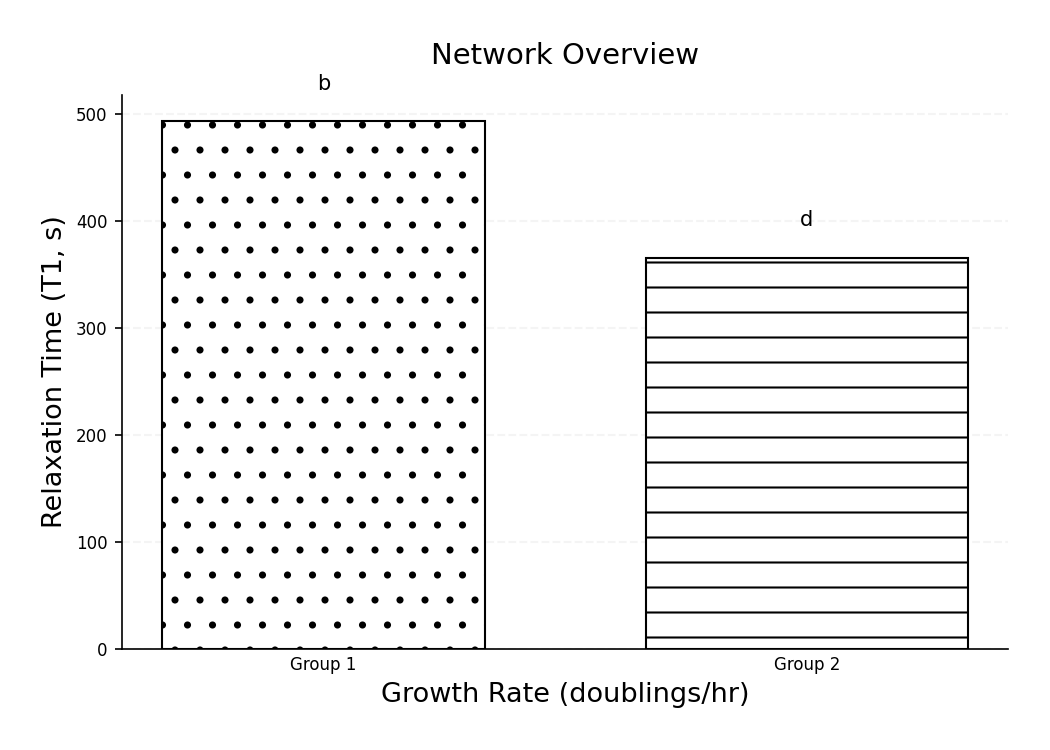
\includegraphics[width=\textwidth]{figures/fig_bar.png}
    \caption{Bar Chart}
    \label{fig:chart_bar}
  \end{subfigure}
  \hfill
  \begin{subfigure}[b]{0.24\textwidth}
    \centering
    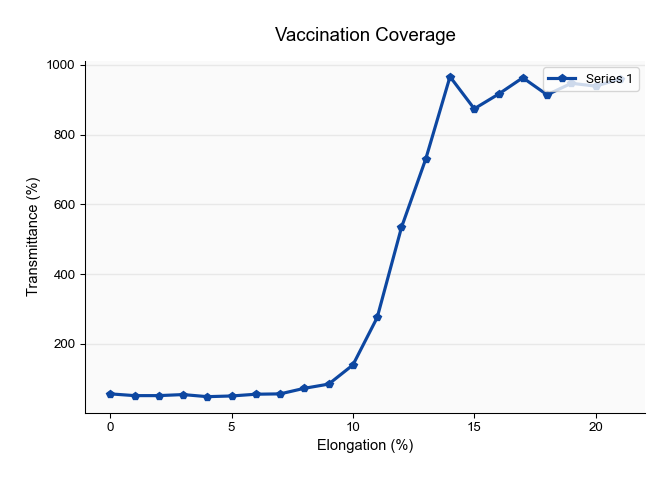
\includegraphics[width=\textwidth]{figures/fig_line.png}
    \caption{Line Chart}
    \label{fig:chart_line}
  \end{subfigure}
  \hfill
  \begin{subfigure}[b]{0.24\textwidth}
    \centering
    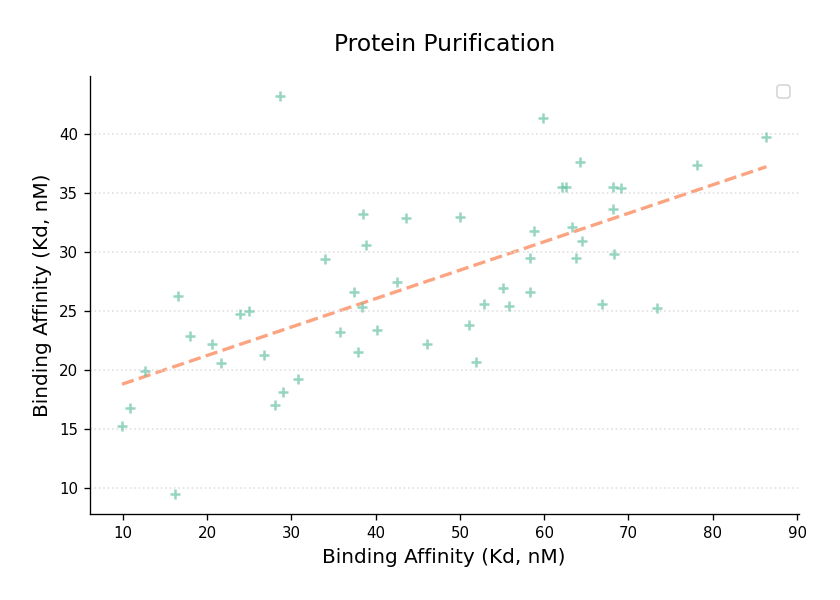
\includegraphics[width=\textwidth]{figures/fig_scatter.png}
    \caption{Scatter Chart}
    \label{fig:chart_scatter}
  \end{subfigure}
  \hfill
  \begin{subfigure}[b]{0.24\textwidth}
    \centering
    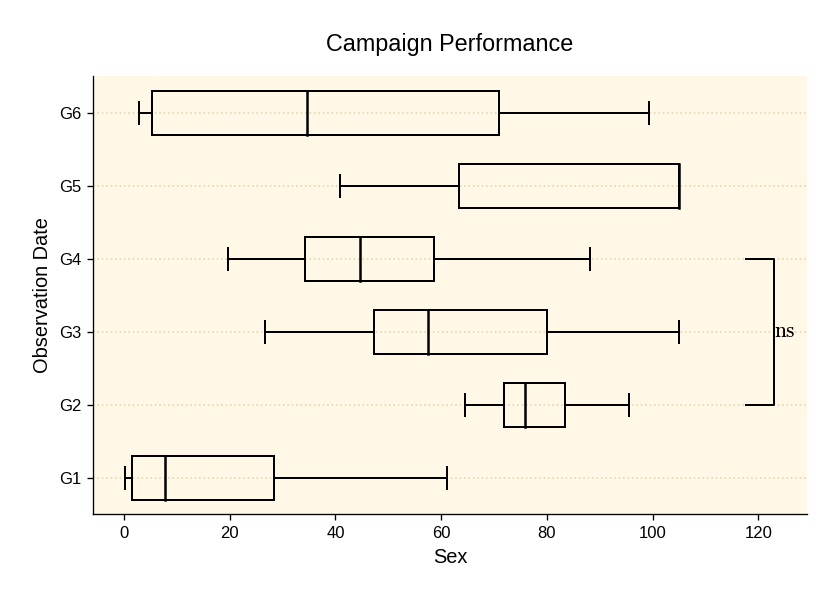
\includegraphics[width=\textwidth]{figures/fig_box.png}
    \caption{Box Plot}
    \label{fig:chart_box}
  \end{subfigure}
  \vskip\baselineskip
  \begin{subfigure}[b]{0.24\textwidth}
    \centering
    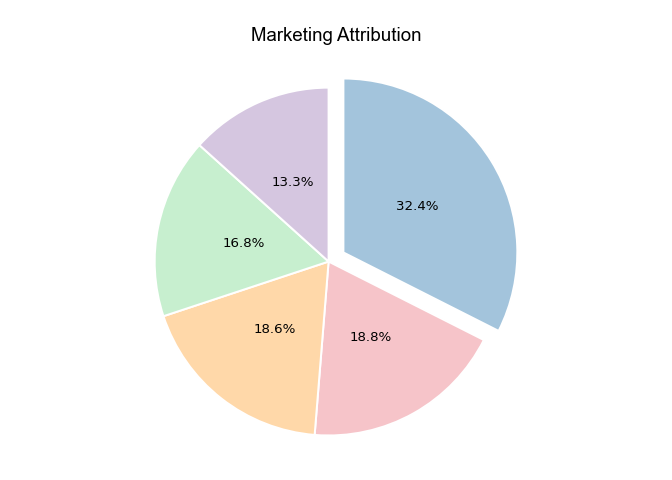
\includegraphics[width=\textwidth]{figures/fig_pie.png}
    \caption{Pie Chart}
    \label{fig:chart_pie}
  \end{subfigure}
  \hfill
  \begin{subfigure}[b]{0.24\textwidth}
    \centering
    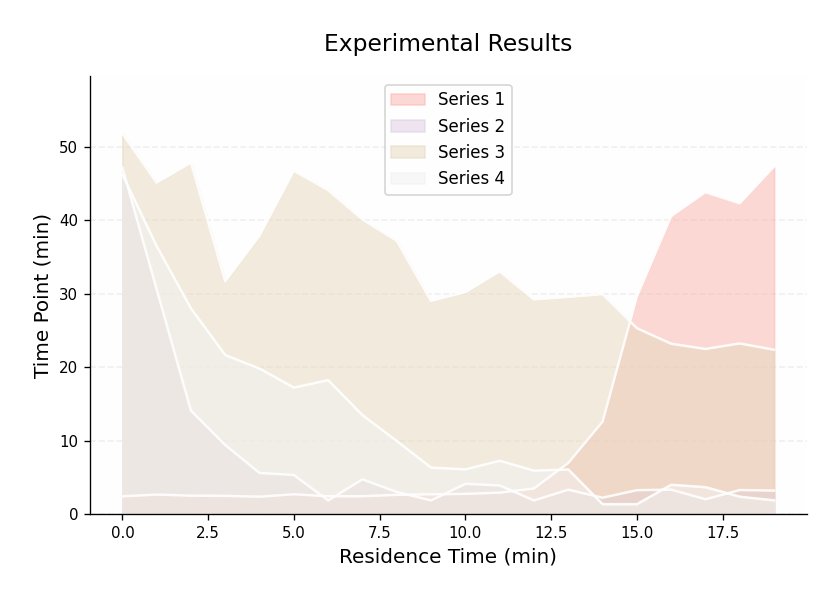
\includegraphics[width=\textwidth]{figures/fig_area.png}
    \caption{Area Chart}
    \label{fig:chart_area}
  \end{subfigure}
  \hfill
  \begin{subfigure}[b]{0.24\textwidth}
    \centering
    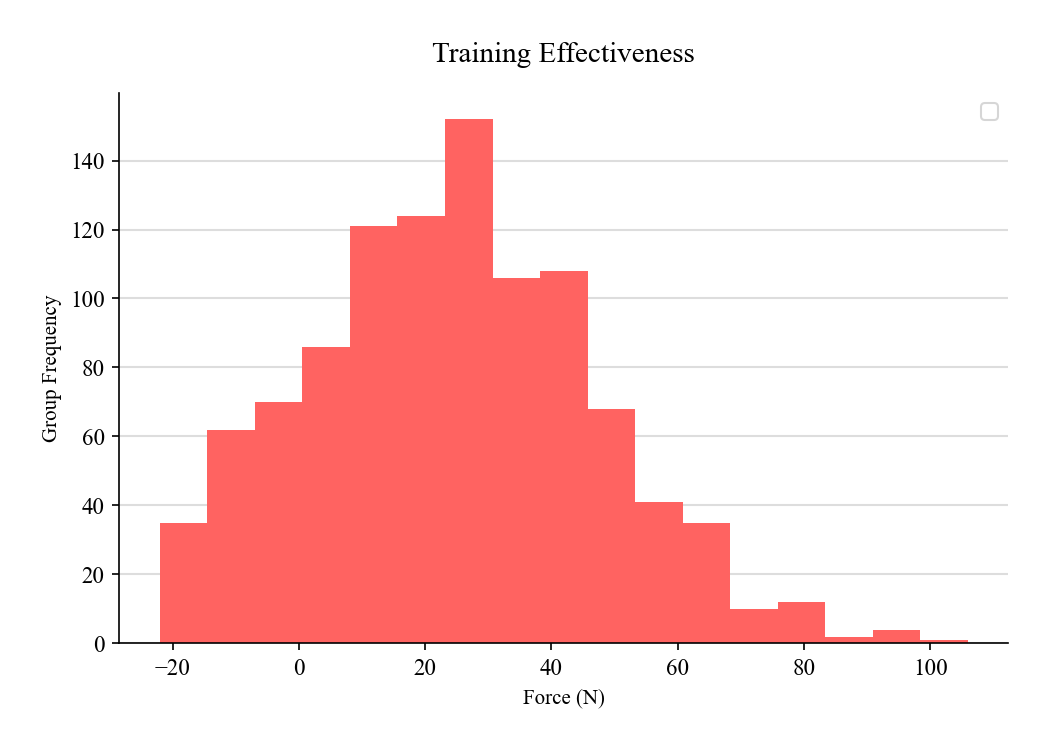
\includegraphics[width=\textwidth]{figures/fig_histogram.png}
    \caption{Histogram}
    \label{fig:chart_histogram}
  \end{subfigure}
  \hfill
  \begin{subfigure}[b]{0.24\textwidth}
    \centering
    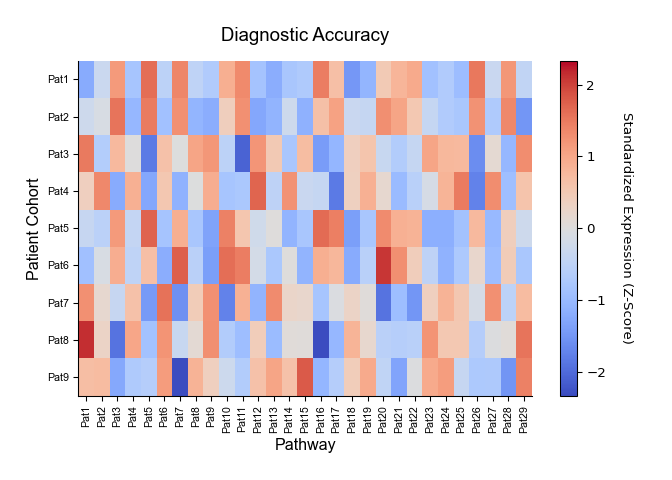
\includegraphics[width=\textwidth]{figures/fig_heatmap.png}
    \caption{Heatmap}
    \label{fig:chart_heatmap}
  \end{subfigure}
  \caption{Layout configurations across the eight chart types produced by the synthesis framework.}
  \label{fig:chart_gallery}
\end{figure*}

\subsection{Dimensional Configurations \& Layout Strategies}\label{sec:configs}

\paragraph{Primary Value Axis.} Switches between vertical and horizontal alignments when category lists exceed 6 groups to preserve label legibility.

\paragraph{Dual Y-Axis Scaling.} Maps distinct datasets onto identical category axes with independent left ($Y_1$) and right ($Y_2$) value scales.

\paragraph{Side-by-Side Grouping.} Arranges multiple series sequentially across categories using an indexed categorical displacement width ($\pm\text{width}/2$).

\paragraph{Stacked Segments.} The baseline coordinate vector for stacked layer $n$ resolves from the preceding cumulative total:
\begin{equation}\label{eq:stacked_bottom}
  \text{bottom}_n = \sum_{i=1}^{n-1} \text{height}_i.
\end{equation}
Cumulative stacking is handled by Matplotlib's~\cite{hunter2007matplotlib} rendering pipeline to maintain geometric consistency under coordinate transforms.

\paragraph{Area Chart Stacking Modes.} Three modes are supported: Overlapping ($\alpha=0.5$, filled from zero baseline), Stacked ($\alpha=0.7$, cumulative sequential layering), and Percentage/Normalized:
\begin{equation}\label{eq:pct_norm}
  y_{k,j} = \frac{y_{\text{raw},k,j}}{\sum_{i=0}^{K-1} y_{\text{raw},i,j} + \epsilon}\times 100.0.
\end{equation}

\paragraph{Hatch Textures.} Geometric patterns (\texttt{none}~= hollow, \texttt{..}~= dotted stipple, \texttt{//}~= diagonal stripes, \texttt{xxxx}~= crossed mesh) are mapped onto patches to retain readability in monochromatic or grayscale domains.

\paragraph{Statistical Significance Overlays.} Step-wise connecting lines drawn over targeted bar pairs, with horizontal beam clearance:
\begin{equation}\label{eq:sig_level}
  \text{level} = \max(\text{envelope})\cdot(1 + p),\quad p \in [0.10,\,0.20].
\end{equation}

\subsection{Bounding Box Resolution and Element Parsing}\label{sec:bbox}

\paragraph{Box Plot Schema (\texttt{CLASS\_MAP\_BOX}).}
The full 10-class contiguous index map ($\{0,\ldots,9\}$) includes generic element classes (\texttt{chart}~=~0, \texttt{axis\_title}~=~2, \texttt{significance\_marker}~=~3, \texttt{legend}~=~5, \texttt{chart\_title}~=~6, \texttt{axis\_labels}~=~8) shared across chart types.
The four box-plot-specific structural classes are:
\begin{itemize}[nosep]
  \item \texttt{box} (Class~1): IQR boundaries ($\text{IQR} = Q_3 - Q_1$).
  \item \texttt{range\_indicator} (Class~4): Union of upper/lower whiskers extending to $1.5\times\text{IQR}$.
  \item \texttt{median\_line} (Class~7): 50th percentile segment.
  A mandatory 3-pixel structural padding layer is applied because single line primitives return zero-area boundaries in raw display buffers.
  \item \texttt{outlier} (Class~9): Points beyond whisker thresholds.
\end{itemize}

\paragraph{Heatmap QuadMesh Parsing.}
For each row $i$ and column $j$, grid vertices are extracted:
\begin{equation}\label{eq:quad_corners}
  \text{Corners} = \bigl[\mathbf{c}_{i,j},\;\mathbf{c}_{i+1,j},\;\mathbf{c}_{i+1,j+1},\;\mathbf{c}_{i,j+1}\bigr].
\end{equation}
Grid vertices pass through \texttt{ax.transData.transform} to yield absolute canvas coordinates, normalized to $[0,1]$ for YOLO exports. Auxiliary color bars are isolated by aspect-ratio filtering ($w/h < 0.3$ vertical, $>3.0$ horizontal).

\subsection{Coordinate Pose Mapping \& Resampling Loops}\label{sec:pose}

\subsubsection{The 5-Keypoint Schema (Pie Charts)}\label{sec:5kpt}

Wedge paths are mapped to a 5-point geometry (\texttt{CLASS\_MAP\_PIE\_POSE}). For exploded slices, the center shifts radially:
\begin{equation}\label{eq:wedge_center}
  \mathbf{c}_{\text{wedge}} = \bigl[\text{explode}\cdot\cos\theta_{\text{mid}},\;\text{explode}\cdot\sin\theta_{\text{mid}}\bigr].
\end{equation}
Intermediate arc coordinates sample at one-third and two-thirds of the angular span:
\begin{equation}\label{eq:arc_interp}
  \theta_{\text{int1}} = \theta_1 + \frac{\theta_2-\theta_1}{3},\quad \theta_{\text{int2}} = \theta_1 + \frac{2(\theta_2-\theta_1)}{3}.
\end{equation}
The five keypoints in display space are: $\mathbf{k}_0$ (wedge center), $\mathbf{k}_1$ and $\mathbf{k}_2$ (start/end arc angles $\theta_1$, $\theta_2$), and $\mathbf{k}_3$, $\mathbf{k}_4$ (interpolated interior positions $\theta_{\text{int1}}$, $\theta_{\text{int2}}$):
\begin{align}
  \mathbf{k}_0 &= [x_c,\; y_c] + \mathbf{c}_{\text{wedge}}, \label{eq:k0}\\
  \mathbf{k}_n &= [x_c + r\cos\theta_n,\; y_c + r\sin\theta_n] \nonumber\\
  &\quad + \mathbf{c}_{\text{wedge}},\; n \in \{1,2,3,4\}, \label{eq:kn}
\end{align}
where $\theta_1$, $\theta_2$ are the start and end angles of the wedge, $\theta_3 \coloneqq \theta_{\text{int1}}$, and $\theta_4 \coloneqq \theta_{\text{int2}} $.

% ============================================================
%  5. AESTHETIC THEMES & POST-RENDERING DEGRADATION
% ============================================================
\section{Aesthetic Themes \& Post-Rendering Degradation Mechanics}\label{sec:themes}

The pipeline decouples visual aesthetics into declarative themes and publication presets before applying post-rendering degradation.

\subsection{Thematic \& Publication Presets}\label{sec:presets}

The style engine (\texttt{themes.py}) configures canvas backdrops, grid visibility, line thicknesses, and typography classes.
Standard styles include:
\begin{itemize}[nosep]
  \item \textbf{excel}: Light-gray background (\texttt{\#F2F2F2}), thick solid white grids ($1.5\,$pt).
  \item \textbf{ggplot}: Dark-gray backdrop (\texttt{\#EBEBEB}), white grids, hidden outer spines.
  \item \textbf{prism}: White background, outward-pointing ticks, sparse dotted grid (\texttt{\#E0E0E0}).
  \item \textbf{retro}: Warm cream canvas (\texttt{\#FFF8E7}), Georgia serif fonts.
\end{itemize}

Publication presets (\texttt{PUBLICATION\_THEMES}) encode journal-specific figure constraints:

\begin{table}[h!]
\centering
\caption{Publication preset configurations.}\label{tab:pub_presets}
\footnotesize
\begin{tabular}{@{} l c c c c c @{}}
\toprule
\textbf{Preset} & \textbf{Size (in)} & \textbf{DPI} & \textbf{Font} & \textbf{Spine} & \textbf{Line}\\
\midrule
\texttt{nature}  & $3.3\!\times\!2.4$ & 300 & 7\,pt & 0.5\,pt & 0.5\,pt\\
\texttt{science} & $3.5\!\times\!2.5$ & 300 & 6\,pt & 0.75\,pt & 0.75\,pt\\
\texttt{cell}    & $6.5\!\times\!4.0$ & 300 & 8\,pt & 0.6\,pt & 0.6\,pt\\
\texttt{lancet}  & $7.0\!\times\!4.5$ & 300 & 8\,pt & 0.8\,pt & 0.8\,pt\\
\texttt{nanotech} & $3.2\!\times\!2.4$ & 600 & 7\,pt & 0.5\,pt & 0.6\,pt\\
\bottomrule
\end{tabular}
\end{table}

\subsection{Post-Rendering Image Degradation Filters}\label{sec:degradation}

Once rendered, images pass through a multi-tiered degradation pipeline (\texttt{effects.py}).
ChartAct~\cite{zhou2026chartact} explores a complementary direction, benchmarking models on sequential action execution over rendered chart canvases.
Figure~\ref{fig:degradation_comparison} compares a clean rendering with its degraded counterpart.

\begin{figure*}[t]
  \centering
  \begin{subfigure}[b]{0.48\textwidth}
    \centering
    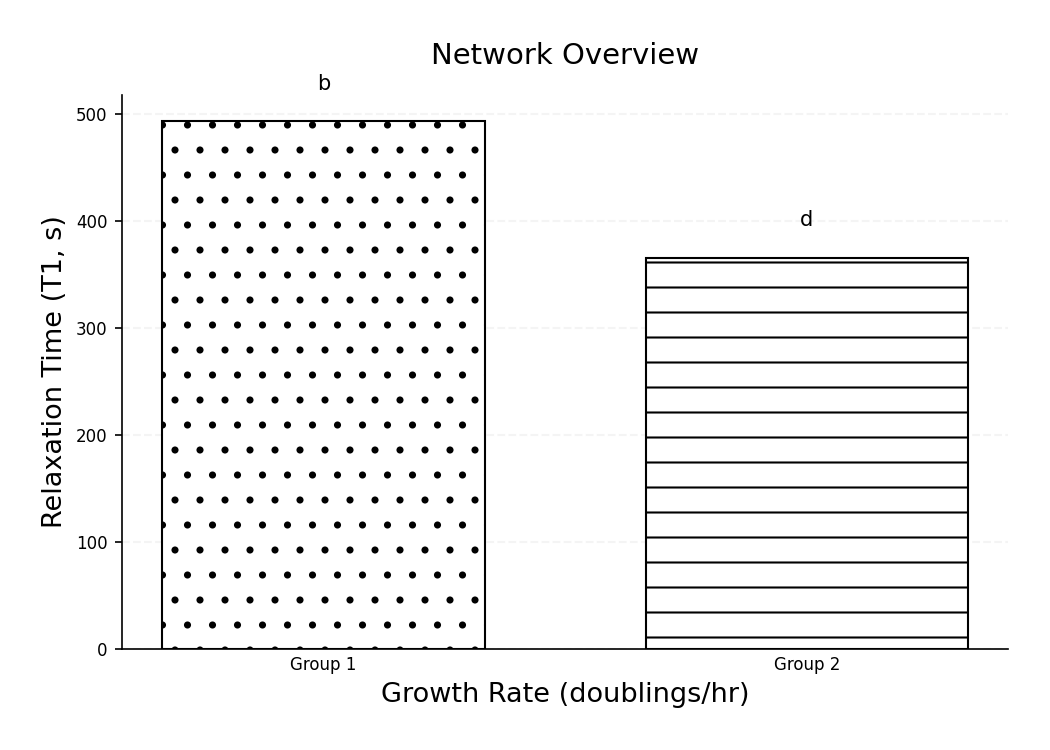
\includegraphics[width=\textwidth]{figures/fig_bar.png}
    \caption{Clean digital vector rendering.}
    \label{fig:degrad_clean}
  \end{subfigure}
  \hfill
  \begin{subfigure}[b]{0.48\textwidth}
    \centering
    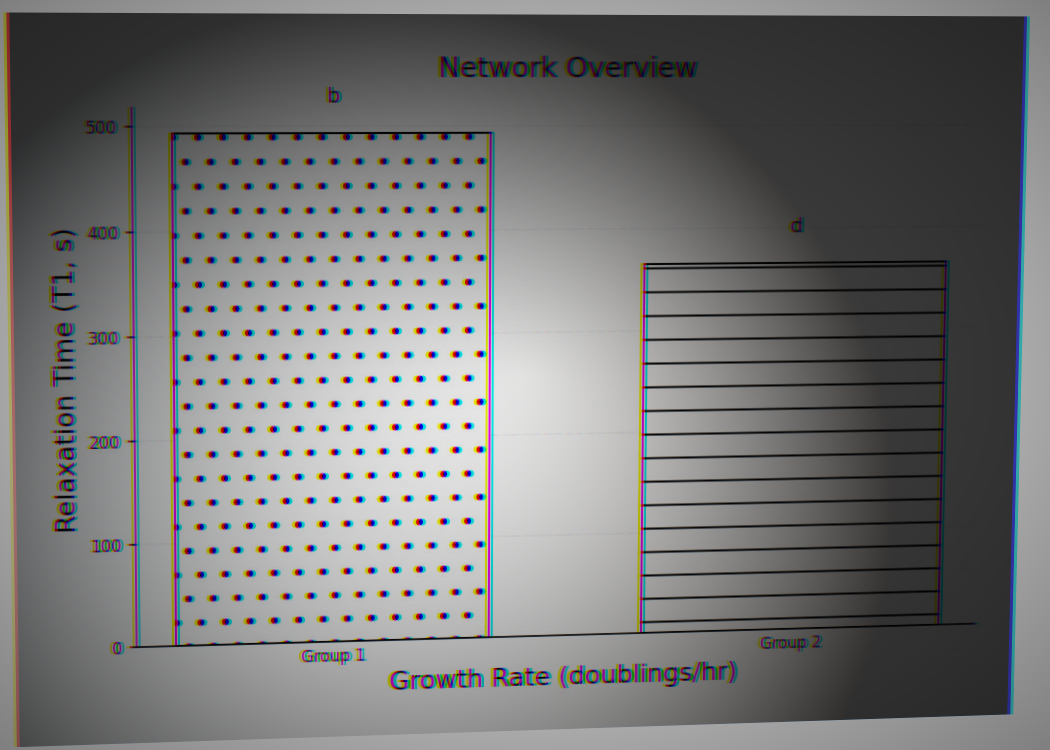
\includegraphics[width=\textwidth]{figures/fig_bar_degraded.png}
    \caption{Degraded canvas following the post-rendering pipeline.}
    \label{fig:degrad_dirty}
  \end{subfigure}
  \caption{Clean rendering (left) versus degraded output (right) after scanner streaks, perspective warping, chromatic aberration, sensor noise, and uneven lighting.}
  \label{fig:degradation_comparison}
\end{figure*}

\subsubsection{General Realism Filters}\label{sec:general_filters}

These filters simulate physical sensor noise and optical degradation following Gonzalez and Woods~\cite{gonzalez2018digital}.

\paragraph{Edge Color Normalization (\texttt{normalize\_edgecolor}).} Darkens patch fill colors in HSV space:
\begin{align}\label{eq:edge_norm}
  V_{\text{new}} &= \max(0,\; V \times 0.6), \nonumber \\
  \text{Edge} &= \text{HSV\_to\_RGB}(H, S, V_{\text{new}}).
\end{align}

\paragraph{Additive White Gaussian Noise (\texttt{apply\_noise\_effect}).}
\begin{equation}\label{eq:awgn}
  I_{\text{noisy}}(x,y,c) = \text{clip}\!\bigl(I_{\text{raw}}(x,y,c) + \text{N}(0,\sigma^2),\; 0,\;255\bigr),
\end{equation}
where $\sigma \sim \mathcal{U}(2.0, 8.0)$.

\paragraph{Directional Motion Blur.} A custom convolution kernel $\mathbf{K}$ models scanner bar movement:
\begin{align}
  x_{\text{idx}} &= \lfloor c + (i-c)\cos\theta\rfloor, \label{eq:motion_idx_x}\\
  y_{\text{idx}} &= \lfloor c + (i-c)\sin\theta\rfloor, \label{eq:motion_idx_y}\\
  \mathbf{K}(y_{\text{idx}}, x_{\text{idx}}) &= 1.0,\quad \mathbf{K}_{\text{norm}} = \mathbf{K}\Big/\!\sum\mathbf{K}. \label{eq:motion_kernel}
\end{align}

\paragraph{Vignette Lighting Falloff (\texttt{apply\_vignette\_effect}).} Quadratic radial attenuation:
\begin{align}
  r(x,y) &= \sqrt{(x-x_c)^2+(y-y_c)^2}, \label{eq:vig_r}\\
  V(x,y) &= \text{clip}\!\biggl(1 - \Bigl(\frac{r}{r_{\max}}\Bigr)^{\!2},\; 0.3,\; 1.0\biggr), \label{eq:vig_V}\\
  I_{\text{final}} &= I \cdot V(x,y). \label{eq:vig_final}
\end{align}

\paragraph{Chromatic Aberration (\texttt{apply\_chromatic\_aberration\_effect}).} Simulates lens dispersion~\cite{boult1992correcting} by shifting Red and Blue channels in opposite directions ($\Delta x, \Delta y$) relative to Green:
\begin{align}
  I_R(x,y) &= I_R(x+\Delta x_r,\; y+\Delta y_r), \label{eq:chrom_r}\\
  I_B(x,y) &= I_B(x+\Delta x_b,\; y+\Delta y_b). \label{eq:chrom_b}
\end{align}

\paragraph{Uneven Lighting (\texttt{apply\_uneven\_lighting\_effect}).} Subtractive radial mask simulating flash hotspots or ambient gradients:
\begin{align}\label{eq:uneven_light}
  M_{\text{radial}}(x,y) &= 1 - \frac{d(x,y)}{\max(d)}\cdot\text{intensity}, \nonumber\\
  &\quad \text{intensity} \in [0,1].
\end{align}

\subsubsection{Resolution and Compression Simulation}\label{sec:resolution}

\paragraph{Camera Downsampling (\texttt{apply\_low\_res\_effect}).} Shrinks via bicubic interpolation and scales back via bilinear: $\text{scale} \sim \mathcal{U}(0.25, 0.60)$.

\paragraph{Pixelation (\texttt{apply\_pixelation\_effect}).} Bilinear downsampling followed by nearest-neighbor upsampling creates block artifacts.

\paragraph{Palette Quantization (\texttt{apply\_posterize\_effect}).} Constrains continuous color depths to $N \in \{16, 32, 64\}$ indexed palette entries.

\subsubsection{Document Scanning \& Physical Overlays}\label{sec:scanning}

\begin{itemize}[nosep]
  \item \textbf{Scanner Streaks}: Semi-transparent horizontal bands at randomized heights simulate dust on a sensor bed.
  \item \textbf{Document Misalignment}: Rotation $\theta \sim \mathcal{U}(-1^\circ, 1^\circ)$.
  \item \textbf{UI Chrome Wrappers}: Desktop browser frames or web tab search bars overlaid at canvas boundaries.
  \item \textbf{Watermarks}: Low-opacity diagonal text stamps (e.g., \textsc{confidential}, \textsc{draft}) at canvas center.
  \item \textbf{Mouse Cursor}: Vector pointer arrow injected at randomized coordinates.
\end{itemize}

\subsubsection{Selective OCR-Targeted Text Degradation}\label{sec:text_degrad}

The module \texttt{apply\_text\_degradation\_effect} isolates textual regions---titles, legends, axis labels---from the scene graph via \texttt{get\_window\_extent}.
Blur and pixelation kernels are applied only within these bounding areas, leaving data curves intact and forcing parsers to learn robust text-recognition patterns.

\subsubsection{The Aesthetic--Quantitative Tension}\label{sec:tension}

Pixel-level filters (vignette, noise, aberration) preserve the coordinate structure of underlying features.
Document rotation (\texttt{apply\_scan\_rotation\_effect}), however, introduces a spatial transform resolved via a 2D rotation about the canvas center:
\begin{equation}\label{eq:rotation_matrix}
  \begin{bmatrix} x' \\ y' \end{bmatrix} = \begin{bmatrix} \cos\theta & \sin\theta \\ -\sin\theta & \cos\theta \end{bmatrix} \begin{bmatrix} x - x_c \\ y - y_c \end{bmatrix} + \begin{bmatrix} x_c \\ y_c \end{bmatrix},
\end{equation}
where $(x_c, y_c)$ is the canvas center. Propagating this transform through the pipeline's coordinate steps (\texttt{transform\_steps}) keeps bounding boxes and keypoint annotations aligned with the rotated canvas.
A similar issue arises with sketch rendering modes (e.g., \texttt{plt.xkcd()}), where jitter introduces non-deterministic element displacement.

\subsection{Homography \& Perspective Warping Mechanics}\label{sec:homography}

The perspective transformation (\texttt{apply\_perspective\_warp\_effect}) maps original corner coordinates to randomized targets shifted inward:
\begin{equation}\label{eq:distortion}
  \Delta x = w \cdot d,\quad \Delta y = h \cdot d,\quad d = 0.08.
\end{equation}

Source coordinates $[x,y]^T$ map to warped targets $[u,v]^T$ via a $3\!\times\!3$ projective matrix following the Direct Linear Transformation (DLT) of Abdel-Aziz and Karara~\cite{abdelaziz1971direct}:
\begin{equation}\label{eq:proj_mat}
  \begin{bmatrix} u \\ v \\ 1\end{bmatrix} \sim
  \begin{bmatrix} h_1 & h_2 & h_3 \\ h_4 & h_5 & h_6 \\ h_7 & h_8 & 1\end{bmatrix}
  \begin{bmatrix} x \\ y \\ 1\end{bmatrix}.
\end{equation}

The eight unknown parameters are solved by expanding four corner mappings into $A\mathbf{h} = \mathbf{b}$:
\begin{equation}\label{eq:homography_system}
  \left[\setlength{\arraycolsep}{3.5pt}\begin{array}{cccccccc}
    x_i & y_i & 1 & 0 & 0 & 0 & -u_i x_i & -u_i y_i\\
    0 & 0 & 0 & x_i & y_i & 1 & -v_i x_i & -v_i y_i
  \end{array}\right]
  \mathbf{h} = \begin{bmatrix} u_i \\ v_i\end{bmatrix}.
\end{equation}
The eight unknowns are recovered via least squares:
\begin{equation}\label{eq:ls_solve}
  \mathbf{h} = (A^\top A)^{-1} A^\top \mathbf{b}.
\end{equation}

The inverse $H^{-1}$ is used for pixel interpolation.
When OpenCV is available, the system calls \texttt{cv2.getPerspectiveTransform}; otherwise it falls back to the algebraic solver.
Ground-truth labels are projected via $H$:
\begin{equation}\label{eq:label_warp}
  \begin{bmatrix} x_w \\ y_w \\ w\end{bmatrix} = H \begin{bmatrix} x_o \\ y_o \\ 1\end{bmatrix},\quad
  \mathbf{p}_{\text{final}} = \biggl[\frac{x_w}{w},\;\frac{y_w}{w}\biggr].
\end{equation}

Cropping offsets from \texttt{apply\_clipping\_effect} apply additive coordinate adjustments:
\begin{equation}\label{eq:clip_adjust}
  x_{\text{adj}} = x_o + \Delta x,\quad y_{\text{adj}} = y_o + \Delta y.
\end{equation}

% ============================================================
%  6. EMPIRICAL EVALUATION & BENCHMARK VALIDATION
% ============================================================
\section{Empirical Evaluation \& Benchmark Validation}\label{sec:evaluation}

We validate the synthetic data by training element-detection networks across all eight chart types.

\subsection{Experimental Setup}\label{sec:setup}

For each chart format, a synthetic corpus is generated with randomized themes, label configurations, and the full degradation suite (motion blur, sensor noise, perspective warping, scanner streaks, vignette falloff). Specifically, each heatmap model is trained on a corpus of 1,200/600 (75\%/25\%) train/validation images, while other graph formats utilize a corpus of 3,600/1,200 (75\%/25\%) train/validation images. The sole exception is the bar plot, which has 3,600/1,200 synthetic graphs supplemented by 351 real graphs annotated manually. The Hugging Face dataset\footnote{\url{https://huggingface.co/datasets/utcz/Plots/tree/main}} is a representative example of the generator.

Detection networks are trained to locate chart primitives---bars, boxes, wedges, data points---as well as axis labels, legends, titles, significance markers, and error bars. All models are trained on the latest YOLO11 model with varying epochs, running for at least 80 epochs each.

\subsection{Results and Performance Analysis}\label{sec:results}

Performance is measured by class-wise Average Precision (AP) and Mean Average Precision at IoU 0.5 (mAP@0.5). Table~\ref{tab:evaluation_results} reports global mAP across ten configurations; Table~\ref{tab:class_ap} provides per-class AP breakdowns for three models with the widest performance spread.

\begin{table}[htbp]
\centering
\caption{Global mAP@0.5 per detection model on degraded synthetic charts.}\label{tab:evaluation_results}
\small
\begin{tabular}{l c c}
\toprule
\textbf{Model} & \textbf{Classes} & \textbf{mAP@0.5} \\
\midrule
Heatmap Lattice    & 2  & 0.855 \\
Heatmap Macro      & 2  & 0.995 \\
Heatmap Text       & 3  & 0.995 \\
Heatmap Color Bar  & 3  & 0.995 \\
Bar Plot           & 8  & 0.976 \\
Box Plot           & 8  & 0.919 \\
Histogram          & 5  & 0.949 \\
Line Plot          & 7  & 0.859 \\
Pie Chart          & 5  & 0.974 \\
Scatter Plot       & 4  & 0.973 \\
\bottomrule
\end{tabular}
\end{table}

\begin{table*}[htbp]
\centering
\caption{Per-class Average Precision breakdown for selected models (mAP@0.5).}\label{tab:class_ap}
\small
\setlength{\tabcolsep}{4pt}
\begin{tabular}{l *{8}{c} c}
\toprule
\textbf{Model} & \multicolumn{8}{c}{\textbf{Class-wise AP}} & \textbf{mAP} \\
\cmidrule(lr){2-9}
\midrule
\textbf{Bar Plot} & bar & ax\_title & sig\_mark & err\_bar & legend & ch\_title & data\_lbl & ax\_lbl & \\
 & .992 & .995 & .942 & .973 & .987 & .995 & .935 & .987 & .976 \\
\addlinespace
\textbf{Box Plot} & box & ax\_title & sig\_mark & rng\_ind & ch\_title & med\_line & ax\_lbl & outlier & \\
 & .995 & .995 & .975 & .995 & .995 & .715 & .983 & .701 & .919 \\
\addlinespace
\textbf{Line Plot} & data\_pt & ax\_title & sig\_mark & legend & ch\_title & data\_lbl & ax\_lbl & & \\
 & .895 & .995 & .236 & .995 & .995 & .913 & .982 & & .859 \\
\bottomrule
\end{tabular}
\end{table*}

Structural text elements (titles, axis labels, legends) and macroscopic layouts (heatmap grids, color bars) consistently exceed 0.990 AP. Performance drops on fine-grained elements under aggressive degradation, as analyzed below.

% ============================================================
%  7. DISCUSSION
% ============================================================
\section{Discussion}\label{sec:discussion}

\subsection{Coordinate-Space Projection Boundaries (Lie Factor Prerequisites)}\label{sec:liefactor}

Tufte's~\cite{tufte2001} Lie Factor assumes graphic and data dimensions are measured in native linear coordinates:
\begin{equation}\label{eq:lie}
  \text{Lie Factor} = \frac{\Delta\text{Graphic Space}}{\Delta\text{Data Space}}.
\end{equation}
Computing graphical distance from raw canvas pixels introduces systematic bias on non-linear scales. On a log axis spanning $10^0$ to $10^4$, bars covering $[10^2,10^3]$ and $[10^3,10^4]$ occupy identical pixel widths yet correspond to data-space changes of 900 vs.\ 9{,}000---a tenfold error. Correct Lie Factor computation requires inverting the axis transform:
\begin{align}\label{eq:lie_inv}
  \mathbf{p}_{\text{data}} &= \mathbf{T}^{-1}\cdot\mathbf{p}_{\text{pixel}}, \nonumber\\
  \mathbf{T} &= \texttt{ax.transData.transform}.
\end{align}
This inversion eliminates projection bias on logarithmic and other non-linear scales.

\subsection{Degradation Sensitivity in Fine-Grained Features}\label{sec:sensitivity}

Detection sensitivity varies with element scale and complexity (Section~\ref{sec:results}).

Structural elements such as boxes (0.995 AP) and chart backgrounds are robust, but fine-grained features degrade under motion blur and perspective warping. In box plots, median lines (0.715 AP) and outlier points (0.701 AP) suffer from pixel-level occlusion under spatial blurring.

The most severe failure is the significance marker in line plots (0.236 AP). These brackets consist of narrow line segments with small text annotations (\texttt{*}, \texttt{ns}); perspective warping and downsampling erode their structural distinctiveness. This result marks a clear performance boundary for current document intelligence systems and motivates the development of higher-resolution visual encoders.

% ============================================================
%  8. CONCLUSION & FUTURE WORK
% ============================================================
\section{Conclusion \& Future Work}\label{sec:conclusion}

We have presented a code-guided chart synthesis and degradation framework that bridges the domain gap in multimodal document intelligence.
Explicit mathematical data models---sigmoidal Hill curves, log-normal replicate variance, and compositional Aitchison simplex sampling---are mapped directly to graphic layouts, replacing manual annotation.
Post-rendering degradation via perspective homography and rotation transforms simulates real-world scanning artifacts while propagating coordinate updates to bounding boxes and pose schemas.

Future work will integrate the procedural generation engines into reinforcement-learning loops for vision-language architectures, enabling dynamic modulation of layout complexity and degradation intensity to systematically probe model limits in highly degraded visual environments.

% ============================================================
%  REFERENCES
% ============================================================
\begin{thebibliography}{35}

\bibitem{abdelaziz1971direct}
Abdel-Aziz, Y. I., \& Karara, H. M. (1971).
\newblock Direct linear transformation from comparator coordinates into object space coordinates in close-range photogrammetry.
\newblock \emph{Proc.\ ASP/UI Symposium on Close-Range Photogrammetry}, pp.\ 1--18.

\bibitem{aitchison1986statistical}
Aitchison, J. (1986).
\newblock \emph{The Statistical Analysis of Compositional Data}.
\newblock Chapman \& Hall, London.

\bibitem{boult1992correcting}
Boult, T. E., \& Wolberg, G. (1992).
\newblock Correcting chromatic aberrations using image warping.
\newblock \emph{Proc.\ IEEE CVPR}, pp.\ 684--687.

\bibitem{finak2015mast}
Finak, G., McDavid, A., Yajima, M., Deng, K., Gersuk, V., Shalek, A. K., Slichter, C. K., Miller, H. W., McElrath, M. J., Prlic, M., Linsley, P. S., \& Gottardo, R. (2015).
\newblock MAST: a flexible statistical framework for assessing cell-specific differences in single-cell RNA-seq gene expression data.
\newblock \emph{Genome Biology}, 16, p.\ 278.

\bibitem{gonzalez2018digital}
Gonzalez, R. C., \& Woods, R. E. (2018).
\newblock \emph{Digital Image Processing} (4th ed.).
\newblock Pearson.

\bibitem{han2026encqa}
Han, S. et al. (2026).
\newblock EncQA: Benchmarking Vision-Language Models on Visual Encodings for Charts.
\newblock \emph{IEEE Transactions on Visualization and Computer Graphics} [Preprint/Early Access].

\bibitem{he2016resnet}
He, K., Zhang, X., Ren, S., \& Sun, J. (2016).
\newblock Deep residual learning for image recognition.
\newblock \emph{Proc.\ IEEE CVPR}, pp.\ 770--778.
\newblock DOI: 10.1109/CVPR.2016.90

\bibitem{hill1910dissociation}
Hill, A. V. (1910).
\newblock The possible effects of the aggregation of the molecules of haemoglobin on its dissociation curves.
\newblock \emph{The Journal of Physiology}, 40(1), pp.\ iv--vii.

\bibitem{hunter2007matplotlib}
Hunter, J.~D. (2007).
\newblock Matplotlib: A 2D graphics environment.
\newblock \emph{Computing in Science \& Engineering}, 9(3), pp.\ 90--95.
\newblock DOI: 10.1109/MCSE.2007.55

\bibitem{kondic2026chartnet}
Kondic, J. (2026).
\newblock ChartNet: A million-scale, high-quality multimodal dataset for robust chart understanding.
\newblock \emph{arXiv preprint arXiv:2603.27064}.

\bibitem{kondic2025chartgen}
Kondic, J. et al. (2025).
\newblock ChartGen: Scaling Chart Understanding Via Code-Guided Synthetic Chart Generation.
\newblock \emph{arXiv preprint arXiv:2507.02424}.

\bibitem{li2024synthesize}
Li, Z., Jasani, B., Tang, P., \& Ghadar, S. (2024).
\newblock Synthesize step-by-step: Tools, templates and LLMs as data generators for reasoning-based chart VQA.
\newblock \emph{Proc.\ IEEE/CVF CVPR}, pp.\ 13613--13623.
\newblock DOI: 10.1109/cvpr52733.2024.01292

\bibitem{lilly2012immunoassay}
Eli Lilly \& Company, \& National Center for Advancing Translational Sciences. (2012).
\newblock Immunoassay Methods.
\newblock In \emph{Assay Guidance Manual}. National Institutes of Health.

\bibitem{limpert2001lognormal}
Limpert, E., Stahel, W. A., \& Abbt, M. (2001).
\newblock Log-normal distributions across the sciences: Keys and clues.
\newblock \emph{BioScience}, 51(5), pp.\ 341--352.

\bibitem{liu2026chartmaster}
Liu, C. (2026).
\newblock ChartMaster: Boosting MLLMs for chart analysis through data, perception, and reasoning optimization.
\newblock \emph{OpenReview / ICLR} [Preprint/Early Access].

\bibitem{makgai2021compositional}
Makgai, S., Bekker, A., \& Arashi, M. (2021).
\newblock Compositional data modeling through Dirichlet innovations.
\newblock \emph{Mathematics}, 9(19), p.\ 2477.

\bibitem{martin1941new}
Martin, A. J. P., \& Synge, R. L. M. (1941).
\newblock A new form of chromatogram employing two liquid phases.
\newblock \emph{Biochemical Journal}, 35(12), pp.\ 1358--1368.

\bibitem{masry2024chartgemma}
Masry, A., Thakkar, M., Bajaj, A., Kartha, A., Hoque, E., \& Joty, S. (2024).
\newblock ChartGemma: Visual instruction-tuning for chart reasoning in the wild.
\newblock \emph{arXiv preprint arXiv:2407.04172}.

\bibitem{masry2025chartqapro}
Masry, A. et al. (2025).
\newblock ChartQAPro: A New Benchmark for Complex Chart Question Answering.
\newblock \emph{Findings of the Association for Computational Linguistics (ACL)}.

\bibitem{meldrum2025newmoney}
Meldrum, J., Suleiman, B., Rabhi, F., \& Alibasa, M.~J. (2025).
\newblock New money: A systematic review of synthetic data generation for finance.
\newblock \emph{arXiv preprint arXiv:2510.26076}.

\bibitem{michaelis1913kinetik}
Michaelis, L., \& Menten, M. L. (1913).
\newblock Die Kinetik der Invertinwirkung.
\newblock \emph{Biochemische Zeitschrift}, 49, pp.\ 333--369.

\bibitem{peng2024dreamstruct}
Peng, Y.-H., Huq, F., Jiang, Y., Wu, J., Li, X.~Y., Bigham, J.~P., \& Pavel, A. (2024).
\newblock DreamStruct: Understanding slides and user interfaces via synthetic data generation.
\newblock \emph{LNCS}, pp.\ 466--485.
\newblock DOI: 10.1007/978-3-031-72691-0\_26

\bibitem{pearson1897mathematical}
Pearson, K. (1897).
\newblock Mathematical contributions to the theory of evolution. On a form of spurious correlation which may arise when indices are used in the measurement of organs.
\newblock \emph{Proc.\ Royal Society of London}, 60, pp.\ 489--498.

\bibitem{rodriguez2025starvector}
Rodriguez, J. et al. (2025).
\newblock From Charts to Code: A Hierarchical Benchmark for Multimodal Models.
\newblock \emph{OpenReview / Structural Vision Workshop}.

\bibitem{rodbard1974statistical}
Rodbard, D. (1974).
\newblock Statistical quality control and routine data processing for radioimmunoassays and immunoradiometric assays.
\newblock \emph{Clinical Chemistry}, 20(10), pp.\ 1255--1270.

\bibitem{sethuraman1994constructive}
Sethuraman, J. (1994).
\newblock A constructive definition of Dirichlet priors.
\newblock \emph{Statistica Sinica}, 4(2), pp.\ 639--650.



\bibitem{suh2025chart2text}
Suh, S. et al. (2025).
\newblock Chart2Text-Enriched: Towards Fine-Grained and Context-Aware Chart Summarization.
\newblock \emph{IEEE Transactions on Visualization and Computer Graphics}.

\bibitem{tufte2001}
Tufte, E.~R. (2001).
\newblock \emph{The Visual Display of Quantitative Information} (2nd ed.).
\newblock Graphics Press, Cheshire, CT.
\newblock ISBN: 0-9613921-4-2

\bibitem{wang2025chainoffunctions}
Wang, X. et al. (2025).
\newblock Chain of Functions: A Programmatic Pipeline for Fine-Grained Chart Reasoning Data Generation.
\newblock \emph{arXiv / ACL Anthology}.

\bibitem{waskom2021seaborn}
Waskom, M.~L. (2021).
\newblock seaborn: statistical data visualization.
\newblock \emph{Journal of Open Source Software}, 6(60), p.\ 3021.
\newblock DOI: 10.21105/joss.03021

\bibitem{yang2025chartmimic}
Yang, Z. et al. (2025).
\newblock ChartMimic: Evaluating LMMs' Code Generation Elements via Visual Mimicking.
\newblock \emph{arXiv preprint arXiv:2501.03152}.

\bibitem{zhou2026chartact}
Zhou, M. et al. (2026).
\newblock ChartAct: A Benchmark for Dynamic Chart Understanding.
\newblock \emph{arXiv preprint arXiv:2605.26994} [Preprint/Early Access].

\end{thebibliography}

\end{document}